\chapter{The Quantum Harmonic Oscillator}

The harmonic oscillator is one of the last indispensable examples in elementary quantum mechanics, and it is worth doing carefully because it is far more than a spring with a mass attached to it. The same mathematics reappears whenever a system has a stable equilibrium and we disturb it only slightly. That is the order of the lecture: first the broad physical motivation, then the classical oscillator, then quantization, then the question of why only special energies are allowed, and only after that the algebraic machinery that generates the full spectrum.

\paragraph{Credit.} These notes follow Leonard Susskind's lecture closely. The preserved blackboard frames included here are retained as documentary support for the derivation, with credit to Leonard Susskind, LazyingArt LLC, and Video2Book.

\section{Why This System Matters}

We begin with a point Susskind emphasizes from the start: the harmonic oscillator is not important because a visible laboratory spring is itself a dramatic quantum system. For an ordinary macroscopic spring, quantum effects are negligible. The importance is that the oscillator is the universal local model near stable equilibrium.

A weight hanging from a spring is the obvious example, but the lecture quickly widens the field. A point on a passing wave oscillates up and down. A sound wave at fixed frequency oscillates. Molecular vibrations oscillate about equilibrium positions. More generally, if a one-dimensional potential has a minimum at some point \(x_{0}\), then near that minimum the potential is well approximated by a quadratic function:
\begin{equation}
V(x)\approx V(x_{0})+\frac{1}{2}V''(x_{0})(x-x_{0})^{2}.
\end{equation}
Thus, whenever there is a stable point and we study small deviations away from it, the harmonic oscillator appears.

This is why quantizing the oscillator pays off broadly. We are not learning a curiosity; we are learning a template.

\section{From Spring Sketch to the Classical Equation of Motion}

The lecture begins concretely, with a mass hanging from a spring and oscillating about its equilibrium position. Susskind chooses the displacement away from equilibrium as the dynamical variable and simply calls it \(x\), even though in the sketch it is drawn vertically.

\begin{figure}[ht]
\centering

\includegraphics[width=0.72\textwidth]{lecture_10_figure_02.png}
\caption{Spring-mass oscillator and the quadratic Lagrangian term.}
\label{fig:ho_classical_board}
\end{figure}

\begin{figure}[ht]
\centering
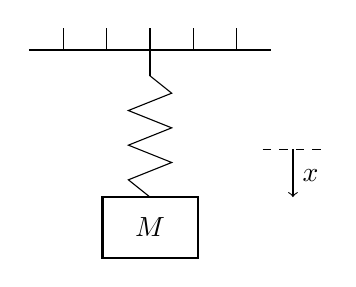
\begin{tikzpicture}[scale=1.1]
\draw[thick] (-1.4,2.6)--(1.4,2.6);
\draw (-1.0,2.6)--(-1.0,2.85);
\draw (-0.5,2.6)--(-0.5,2.85);
\draw (0.0,2.6)--(0.0,2.85);
\draw (0.5,2.6)--(0.5,2.85);
\draw (1.0,2.6)--(1.0,2.85);
\draw (0,2.6)--(0,2.3);
\draw (0,2.3)--(0.25,2.1)--(-0.25,1.9)--(0.25,1.7)--(-0.25,1.5)--(0.25,1.3)--(-0.25,1.1)--(0,0.9);
\draw[thick] (-0.55,0.2) rectangle (0.55,0.9);
\node at (0,0.55) {\(M\)};
\draw[dashed] (1.3,1.45)--(2.0,1.45);
\draw[->] (1.65,1.45)--(1.65,0.9);
\node[right] at (1.65,1.15) {\(x\)};
\end{tikzpicture}
\caption{A clean redraw of the spring-mass picture used in the classical setup.}
\label{fig:ho_classical_tikz}
\end{figure}

The first simplifying move is to absorb the mass into the coordinate. If the original displacement is \(x_{\mathrm{old}}\), then one may introduce
\begin{equation}
y=\sqrt{m}\,x_{\mathrm{old}},
\qquad
\dot y^{\,2}=m\,\dot x_{\mathrm{old}}^{\,2}.
\end{equation}
After this rescaling, Susskind simply renames the new coordinate \(x\). He then chooses the spring constant to be \(\omega^{2}\). With those conventions, the Lagrangian takes the standard form
\begin{equation}
L=\frac{1}{2}\dot x^{2}-\frac{1}{2}\omega^{2}x^{2}.
\end{equation}

The canonical momentum conjugate to \(x\) is immediate:
\begin{equation}
p=\frac{\partial L}{\partial \dot x}=\dot x.
\end{equation}
Applying the Euler--Lagrange equation,
\begin{equation}
\frac{d}{dt}\frac{\partial L}{\partial \dot x}
=
\frac{\partial L}{\partial x},
\end{equation}
we obtain
\begin{equation}
\ddot x=-\omega^{2}x.
\end{equation}
The minus sign is physically the restoring sign: if we displace the oscillator one way, the force points back toward equilibrium.

The classical motion is therefore
\begin{equation}
x(t)=a\cos\omega t+b\sin\omega t.
\end{equation}
That closes the classical setup. Only now do we turn to the quantum problem.

\section{Quantization: States, Operators, and the Hamiltonian}

The lecture insists on a particular order. Before discussing the Hamiltonian, we first need a space of states. For a particle moving on a line, the states are wave functions \(\psi(x)\), with probability density
\begin{equation}
|\psi(x)|^{2}=\psi^{*}(x)\psi(x).
\end{equation}
The variable \(x\) is now both a coordinate and, in quantum mechanics, an observable represented by an operator acting on wave functions. Its action is multiplication:
\begin{equation}
\hat x\,\psi(x)=x\,\psi(x).
\end{equation}
The momentum operator is represented, with \(\hbar=1\) for the moment, by
\begin{equation}
\hat p\,\psi(x)=-i\frac{\partial \psi}{\partial x}.
\end{equation}

On the classical side, the Hamiltonian is
\begin{equation}
H=p\dot x-L.
\end{equation}
Since \(p=\dot x\), this becomes
\begin{equation}
H=\frac{1}{2}p^{2}+\frac{1}{2}\omega^{2}x^{2}.
\end{equation}

\begin{figure}[ht]
\centering

\includegraphics[width=0.72\textwidth]{lecture_10_figure_03.png}
\caption{Hamiltonian rewritten as an operator on the wave function.}
\label{fig:ho_hamiltonian_board}
\end{figure}

Once we replace \(x\) and \(p\) by operators, the Hamiltonian acts on wave functions as
\begin{align}
H\psi(x)
&=
\frac{1}{2}\hat p^{\,2}\psi(x)+\frac{1}{2}\omega^{2}x^{2}\psi(x) \\
&=
-\frac{1}{2}\frac{\partial^{2}\psi}{\partial x^{2}}
+\frac{1}{2}\omega^{2}x^{2}\psi(x).
\end{align}
That is the quantum Hamiltonian of the oscillator in the \(x\)-representation.

\section{Two Uses of the Hamiltonian and the Energy Eigenvalue Problem}

At this stage Susskind pauses to separate two uses of the Hamiltonian. One is dynamical: it tells us how the state changes with time. The other is spectral: it tells us the allowed energies.

The time-dependent Schr\"odinger equation is
\begin{equation}
i\frac{\partial \psi(x,t)}{\partial t}=H\psi(x,t).
\end{equation}
Substituting the oscillator Hamiltonian gives
\begin{equation}
i\frac{\partial \psi}{\partial t}
=
-\frac{1}{2}\frac{\partial^{2}\psi}{\partial x^{2}}
+\frac{1}{2}\omega^{2}x^{2}\psi.
\end{equation}
This explains why the wave function must in general be complex: even if \(\psi(x,0)\) were real at one instant, the factor of \(i\) in the evolution equation immediately produces an imaginary part.

But the lecture then deliberately narrows the discussion. Instead of solving the full time-dependent problem, we focus on energy eigenvectors:
\begin{equation}
H\psi_{E}(x)=E\,\psi_{E}(x).
\end{equation}
In explicit form,
\begin{equation}
-\frac{1}{2}\psi_{E}''(x)+\frac{1}{2}\omega^{2}x^{2}\psi_{E}(x)=E\,\psi_{E}(x).
\label{eq:ho_tise}
\end{equation}

Why does this equation not allow every value of \(E\)? The lecture answers this in a way that is mathematically elementary but physically sharp. Equation \eqref{eq:ho_tise} is second order, so for generic \(E\) there are two linearly independent solutions. At large \(|x|\), the quadratic potential dominates, and the solutions behave qualitatively like a linear combination of a decaying Gaussian-type piece and a growing Gaussian-type piece:
\begin{equation}
\psi(x)\sim \exp\!\left(-\frac{\omega x^{2}}{2}\right)
\quad\text{or}\quad
\psi(x)\sim \exp\!\left(+\frac{\omega x^{2}}{2}\right),
\qquad |x|\to\infty,
\end{equation}
up to subleading corrections and overall factors.

The growing piece is unacceptable. It sends the probability density outward instead of concentrating it in finite space, and in a confining potential it corresponds to pushing the system into a region of arbitrarily large potential energy. Thus the true state space is not all formal solutions of the differential equation but the square-integrable ones:
\begin{equation}
\int_{-\infty}^{\infty} |\psi(x)|^{2}\,dx=1.
\end{equation}
Only for special values of \(E\) does the growing component disappear in both directions. Those special values are the discrete energy levels.

\section{Ground State and Zero-Point Energy}

Before solving the whole spectrum, Susskind looks for one explicit solution. The trial function is the obvious decaying Gaussian,
\begin{equation}
\psi_{0}(x)\propto e^{-\frac{\omega}{2}x^{2}}.
\end{equation}
The normalization is postponed, just as in the lecture. What matters first is whether this wave function is an eigenvector of the Hamiltonian.

\begin{figure}[ht]
\centering

\includegraphics[width=0.82\textwidth]{lecture_10_figure_04.png}
\caption{Gaussian trial state checked as an energy eigenvector.}
\label{fig:ho_gaussian_board}
\end{figure}

The blackboard calculation is partially hard to read in the middle, but the intended algebra is clear. We differentiate once:
\begin{equation}
\psi_{0}'(x)=-\omega x\,\psi_{0}(x).
\end{equation}
Differentiating again,
\begin{equation}
\psi_{0}''(x)=(-\omega+\omega^{2}x^{2})\psi_{0}(x).
\end{equation}
Now act with the Hamiltonian:
\begin{align}
H\psi_{0}
&=
-\frac{1}{2}\psi_{0}''+\frac{1}{2}\omega^{2}x^{2}\psi_{0} \\
&=
-\frac{1}{2}(-\omega+\omega^{2}x^{2})\psi_{0}
+\frac{1}{2}\omega^{2}x^{2}\psi_{0} \\
&=
\left(
\frac{\omega}{2}
-\frac{\omega^{2}x^{2}}{2}
+\frac{\omega^{2}x^{2}}{2}
\right)\psi_{0} \\
&=
\frac{\omega}{2}\psi_{0}.
\end{align}
The \(x^{2}\) terms cancel exactly, which is the crucial payoff of the calculation. Therefore
\begin{equation}
E_{0}=\frac{\omega}{2}.
\end{equation}
Restoring \(\hbar\) at the end, the physical ground-state energy is
\begin{equation}
E_{0}=\frac{\hbar\omega}{2}.
\end{equation}
This is the zero-point energy. Classically one would have expected zero; quantum mechanically the lowest energy is already positive.

\subsection{Question \& Answer}

\paragraph{Why is there no zero-energy state?}

This is the natural local obstacle in the lecture, and Susskind answers it in three linked ways.

\begin{enumerate}
\item First, by the uncertainty principle. Classically we minimize
\(
H=\frac{1}{2}p^{2}+\frac{1}{2}\omega^{2}x^{2}
\)
by setting both \(x\) and \(p\) to zero. Quantum mechanically that is impossible. We can compromise, but we cannot make both vanish sharply. Therefore the ground-state energy cannot be zero.

\item Second, by testing the naive guess \(\psi(x)=1\). This wave function does represent zero momentum, since \(p\) acting on a constant gives zero. But it does not solve the eigenvalue equation:
\begin{equation}
H(1)=\frac{1}{2}\omega^{2}x^{2}\neq 0.
\end{equation}
So \(\psi=1\) does not give a zero-energy eigenstate. It kills the kinetic term, but not the potential term.

\item Third, by the asymptotic behavior of the differential equation. If we set \(E=0\) in
\begin{equation}
-\frac{1}{2}\psi''+\frac{1}{2}\omega^{2}x^{2}\psi=0,
\end{equation}
the solutions do not produce a normalizable state. One may tune initial conditions to make the solution decrease on one side, but then it blows up on the other. Generically it blows up in both directions. Hence \(E=0\) is excluded at the level of admissible wave functions.
\end{enumerate}

\begin{figure}[ht]
\centering

\includegraphics[width=0.58\textwidth]{lecture_10_figure_05.png}
\caption{Harmonic-oscillator Schr\"odinger equation during the \(\psi=1\) discussion.}
\label{fig:ho_zero_energy_board}
\end{figure}

The lecture closes this exchange by making the admissibility condition explicit: the state vectors of the quantum system must be normalizable. That can be taken as an axiom, but the lecture gives the more satisfying explanation as well: a blowing-up solution would place all the probability infinitely far away.

\section{Ladder Operators and the Algebraic Reformulation}

After the break, the method changes. Instead of attacking new eigenfunctions directly by differential equations, the lecture reorganizes the Hamiltonian algebraically.

On the board, Susskind first introduces the unnormalized combinations
\begin{equation}
b_{-}=p-i\omega x,
\qquad
b_{+}=p+i\omega x.
\end{equation}
If \(x\) and \(p\) commuted, we could simply factor the Hamiltonian as a sum of squares. In quantum mechanics they do not commute, and the difference is exactly the source of the zero-point term.

\begin{figure}[ht]
\centering

\includegraphics[width=0.74\textwidth]{lecture_10_figure_06.png}
\caption{Hamiltonian in ladder-operator form.}
\label{fig:ho_ladder_board}
\end{figure}

The lecture itself hesitates over names and signs for a while, but the corrected algebra is straightforward. Using \([x,p]=i\) with \(\hbar=1\),
\begin{align}
b_{+}b_{-}
&=
(p+i\omega x)(p-i\omega x) \\
&=
p^{2}+\omega^{2}x^{2}+i\omega(xp-px) \\
&=
p^{2}+\omega^{2}x^{2}-\omega.
\end{align}
Therefore
\begin{equation}
H=\frac{1}{2}(p^{2}+\omega^{2}x^{2})
=
\frac{1}{2}b_{+}b_{-}+\frac{\omega}{2}.
\end{equation}
The extra \(\omega/2\) is just the zero-point energy found earlier by the Gaussian calculation.

It is then convenient to rescale the operators:
\begin{equation}
a=\frac{1}{\sqrt{2\omega}}(p-i\omega x),
\qquad
a^{\dagger}=\frac{1}{\sqrt{2\omega}}(p+i\omega x).
\end{equation}
These satisfy
\begin{equation}
[a,a^{\dagger}]=1,
\end{equation}
and the Hamiltonian becomes
\begin{equation}
H=\omega\left(a^{\dagger}a+\frac{1}{2}\right).
\label{eq:ho_ladder_H}
\end{equation}

The decisive property of the ground state is now very compact:
\begin{equation}
a\,\psi_{0}=0.
\end{equation}
Indeed,
\begin{align}
a\,\psi_{0}
&=
\frac{1}{\sqrt{2\omega}}\left(-i\frac{d}{dx}-i\omega x\right)e^{-\omega x^{2}/2} \\
&=
-\frac{i}{\sqrt{2\omega}}
\left(
\frac{d}{dx}+\omega x
\right)e^{-\omega x^{2}/2}
=
0,
\end{align}
because
\(
\frac{d}{dx}e^{-\omega x^{2}/2}=-\omega x e^{-\omega x^{2}/2}.
\)
So the algebra already knows the ground state.

\section{Excited States and Physical Meaning}

Once the Hamiltonian is written in the form \eqref{eq:ho_ladder_H}, the spectrum is generated by operator algebra. Let
\begin{equation}
N=a^{\dagger}a
\end{equation}
and suppose
\begin{equation}
N|n\rangle=n|n\rangle.
\end{equation}
Then
\begin{align}
N(a^{\dagger}|n\rangle)
&=
a^{\dagger}a\,a^{\dagger}|n\rangle \\
&=
a^{\dagger}(aa^{\dagger})|n\rangle \\
&=
a^{\dagger}(a^{\dagger}a+1)|n\rangle \\
&=
(n+1)a^{\dagger}|n\rangle.
\end{align}
So \(a^{\dagger}\) raises the eigenvalue of \(N\) by one. By the same reasoning, \(a\) lowers it by one until the ground state is reached, at which point it gives zero.

Thus the energy spectrum is
\begin{equation}
E_{n}=\omega\left(n+\frac{1}{2}\right),
\qquad n=0,1,2,\dots
\end{equation}
or, with \(\hbar\) restored,
\begin{equation}
E_{n}=\hbar\omega\left(n+\frac{1}{2}\right).
\end{equation}

The first excited state is obtained by applying the raising operator once:
\begin{align}
\psi_{1}(x)
&\propto
a^{\dagger}\psi_{0}(x) \\
&=
\frac{1}{\sqrt{2\omega}}
\left(
-i\frac{d}{dx}+i\omega x
\right)e^{-\omega x^{2}/2} \\
&\propto
x\,e^{-\omega x^{2}/2}.
\end{align}
So the first excited wave function is a Gaussian multiplied by \(x\). It vanishes at the origin, and therefore has one node.

This pattern continues. Each time we apply the raising operator, we multiply the Gaussian by a higher polynomial. The result is always of the form
\begin{equation}
\psi_{n}(x)=P_{n}(x)e^{-\omega x^{2}/2},
\end{equation}
with \(P_{n}(x)\) a degree-\(n\) polynomial. The lecture does not develop the full Hermite-polynomial formalism, and it is better not to force it here. The points that matter for this lecture are simpler:

\begin{itemize}
\item each new excitation adds one node;
\item the parity alternates between symmetric and antisymmetric;
\item the wave function oscillates more rapidly as \(n\) grows, indicating larger momentum content;
\item the spatial spread also increases, reflecting larger excursions away from the minimum.
\end{itemize}

This brings the lecture back to interpretation. What does a quantum harmonic oscillator \emph{look like}? In Susskind's formulation, that is the wrong question if one means a literal visual picture. A quantum system is not something we photograph without disturbing it. The right question is what the probability distribution looks like.

For the ground state, the probability density is Gaussian. Its width is controlled by \(\omega\). A larger \(\omega\) means a stiffer restoring force, and therefore a narrower wave function. This is exactly what one expects physically: the tighter the spring, the more strongly the particle is held near the minimum.

The lecture ends by returning to the general rule announced at the beginning. If a system has a stable minimum, then nearby the minimum its potential is approximately quadratic, and the motion is approximately harmonic. That is why diatomic molecules and many other small oscillations are described, at leading order, by this same quantized oscillator.

There is one final structural point worth preserving. The harmonic oscillator is special among equally spaced spectra because it is bounded below. One can invent other equally spaced operators, but if the spectrum runs both upward and downward without bottom, it is not the oscillator. The oscillator is the case with equal spacing \emph{and} a ground state.

\section{Summary}

The lecture builds the quantum harmonic oscillator in two passes. First, starting from the classical Lagrangian, it constructs the Hamiltonian, writes the Schr\"odinger equation, and explains why admissible solutions exist only for discrete energies. Second, it finds the Gaussian ground state explicitly, identifies the zero-point energy \(E_{0}=\hbar\omega/2\), and then reformulates the problem in terms of creation and annihilation operators to generate the full spectrum
\(
E_{n}=\hbar\omega(n+\tfrac{1}{2}).
\)

The payoff is larger than the example itself. Near any stable equilibrium, the world becomes approximately quadratic, and therefore approximately harmonic. Quantizing the oscillator is therefore not the study of a single mechanical gadget. It is the study of the local quantum mechanics of stability itself.